\section*{Aufgabe 1}

\subsection*{a)}

Es sollen das Gradientenverfahren und das konjugierte Gradientenverfahren implementiert und mithilfe der Rosenbrock-Funktion
\begin{equation*}
  f(x_1, x_2) = (1-x_1)^2+100(x_2-x_1^2)^2
\end{equation*}
getestet werden.
Dabei ist der Startpunkt \(\vec{x}_0 = (-1, -1)^{\text{T}}\) und das analytische Minimum beträgt \(\vec{x}_\text{analytisch} = (1,1)^{\text{T}}\).
Das Gradientenverfahren konvergiert nur sehr langsam und erreicht die gewünschte Genauigkeit von \(|g| = \num{0,05}\) erst nach der \(\num{27060837}\)-ten Iteration.
Allerdings ist die Abweichung vom tatsächlichen Minimum mit
\begin{equation*}
  \varepsilon = ||\vec{x}_\text{n} - \vec{x}_\text{analytisch}|| = \num{0,000165825}
\end{equation*}
nur sehr gering.
In Abbildung \ref{fig:grad} sind der Contour-Plot und der Fehler des Gradientenverfahrens aufgetragen.
\begin{figure}
  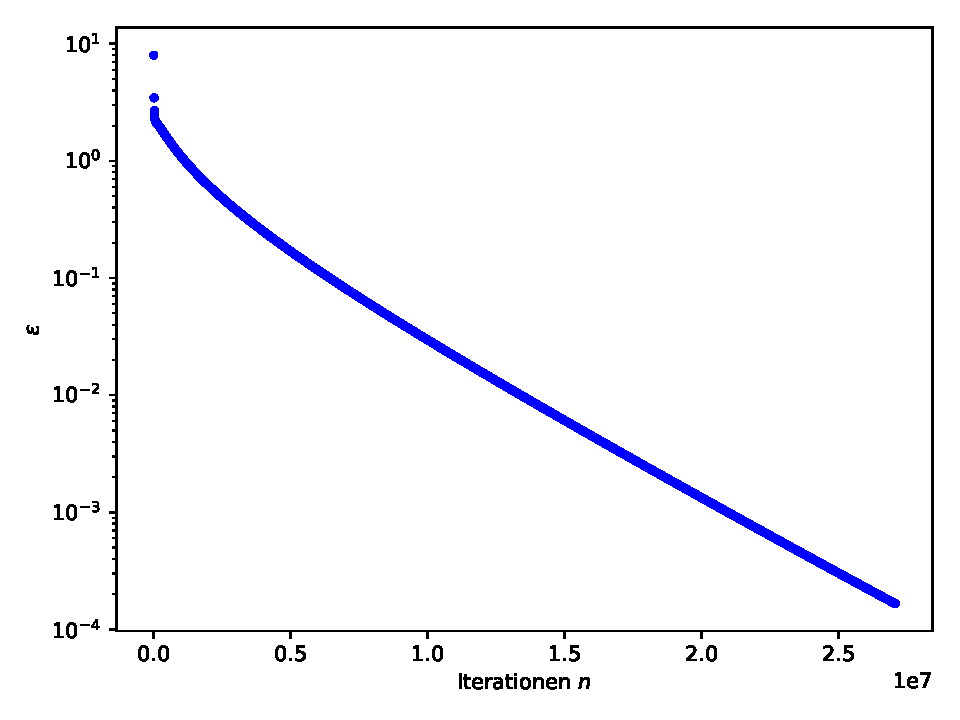
\includegraphics[width=0.45\textwidth]{A1/build/gradientenverfahren.pdf}
  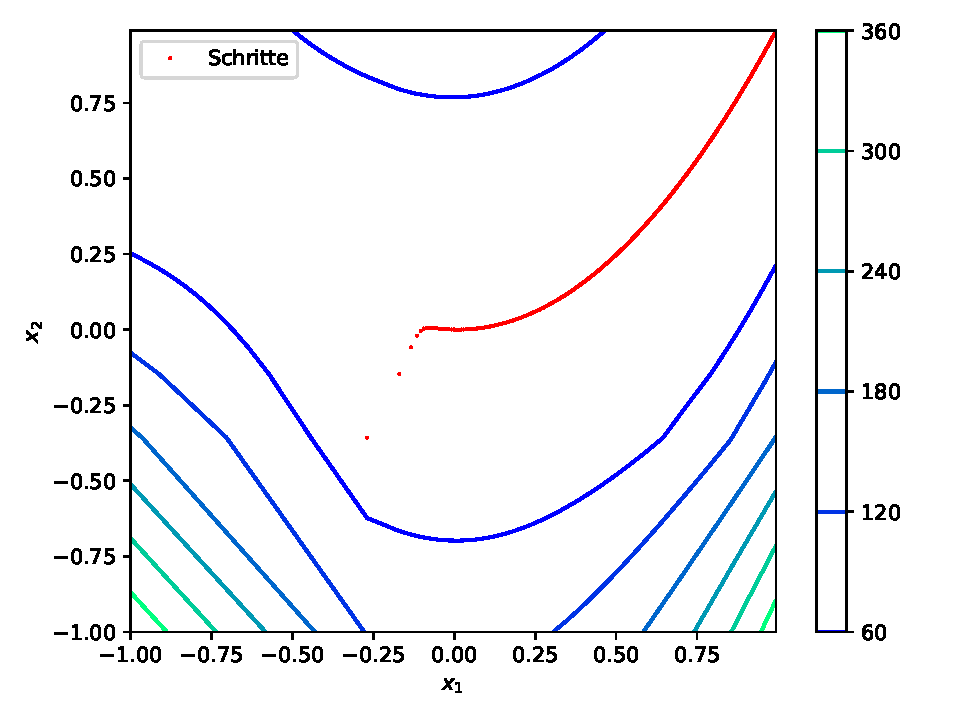
\includegraphics[width=0.45\textwidth]{A1/build/gradientenverfahren_contour.pdf}
  \caption{Fehler- und Contour-Plot beim Gradientenverfahren.}
  \label{fig:grad}
\end{figure}
Das konjugierte Gradientenverfahren fängt bei den letzten drei Iterationen an zu divergieren und wir haben den Fehler leider nicht gefunden. Als Minimum ergibt sich hier nach der \(\num{1333}\)-ten Iteration \(\vec{x} = (\num{2,6232e+14}, \num{4,017e+13})^\text{T}\).
In Aufgabenteil b) stimmen die Ergebnisse des konjugierten Gradientenverfahrens aber mit denen des gewöhnlichen Gradientenverfahrens überein.
In Abbildung \ref{fig:konj_rose} sind der Contour-Plot und der Fehler des konjugierten Gradientenverfahrens ohne die letzten drei Werte dargestellt. Da allerdings bei der Berechnung etwas schief läuft sind diese nur bedingt aussagekräftig.
\begin{figure}
  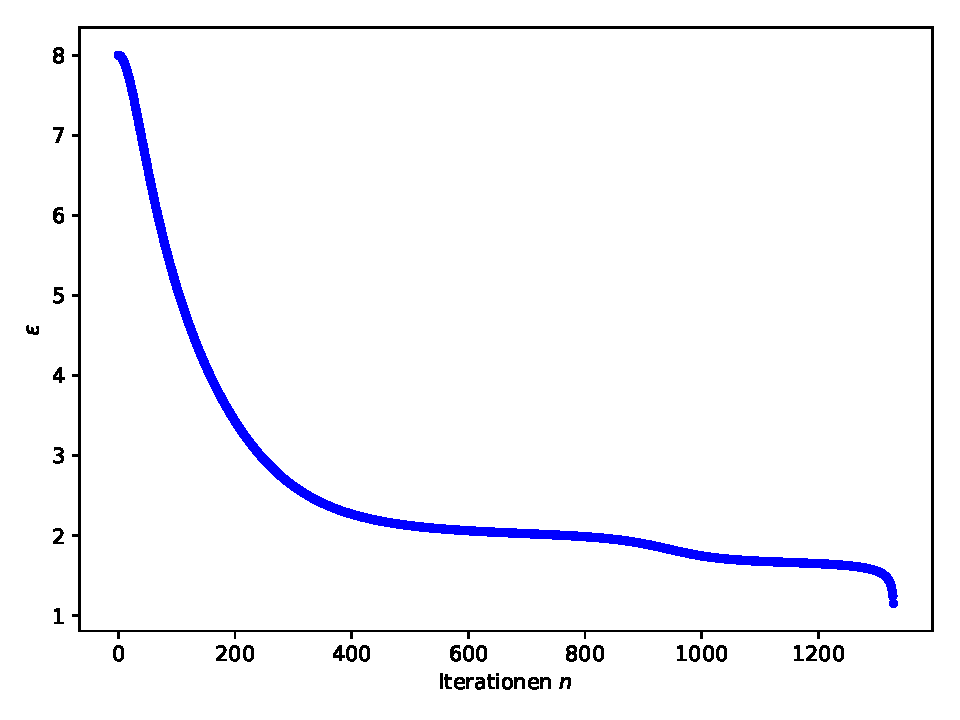
\includegraphics[width=0.45\textwidth]{A1/build/konjugiert_rosenbrock.pdf}
  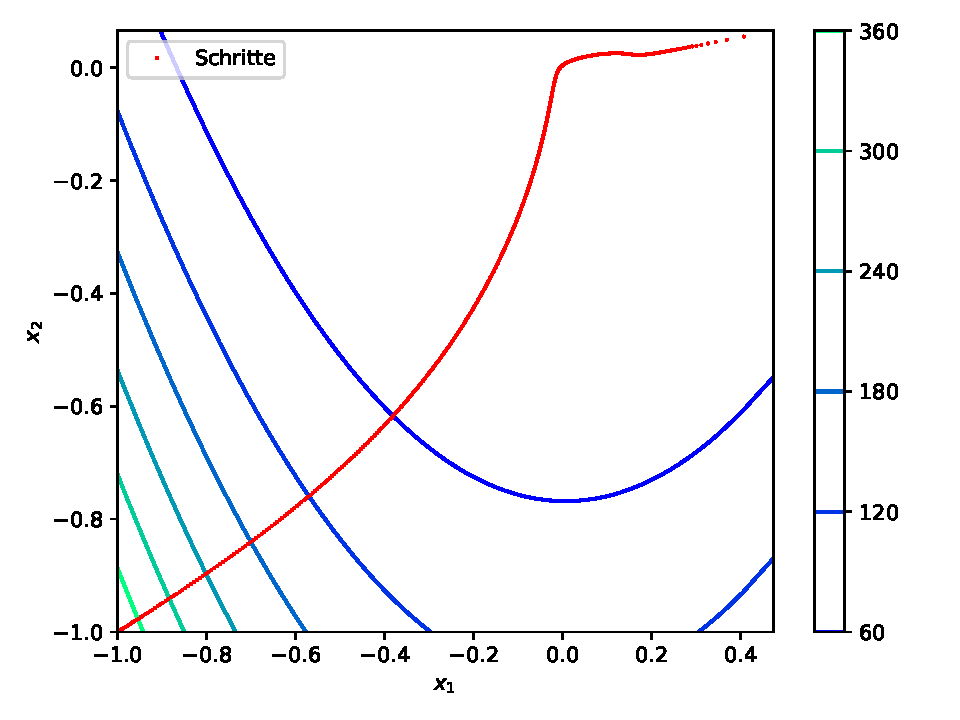
\includegraphics[width=0.45\textwidth]{A1/build/konjugiert_rosenbrock_contour.pdf}
  \caption{Fehler- und Contour-Plot beim konjugierten Gradientenverfahren.}
  \label{fig:konj_rose}
\end{figure}

\FloatBarrier

\subsection*{b)}

Nun sollte das konjugierte Gradientenverfahren auf die Funktion
\begin{equation*}
  f(x) = \frac{1}{1 + \frac{e^{-10(x_1 x_2 - 3)^2}}{x_1^2 + x_2^2}}
\end{equation*}
angewendet werden.
Dabei werden die Ergebnisse für die drei Startpunkte \\ {\(\vec{x}_0 \: \in \: \{(\num{1.5}; \num{2.3})^\text{T}, (\num{-1.7}; \num{-1.9})^\text{T}, (\num{0.5}; \num{0.6})^\text{T} \}\)} ausgewertet.
Für die dritte Startbedingung funktioniert das Verfahren nicht, da der Gradient an dieser Stelle schon so klein ist, dass er auf Null gerundet wird.
Beim ersten Startwert wird nach \(\num{4269}\) Iterationen das Minimum \((\num{1.35728};  \num{2.21221})^\text{T}\) erreicht.
Beim zweiten Startwert ergibt sich nach \(\num{3823}\) Iterationen \((\num{-1.63204};  \num{-1.8397})^\text{T}\).
In Abbildung \ref{fig:contour_b} sind die Contour-Plots für die ersten beiden Startwerte dargestellt.
\begin{figure}
  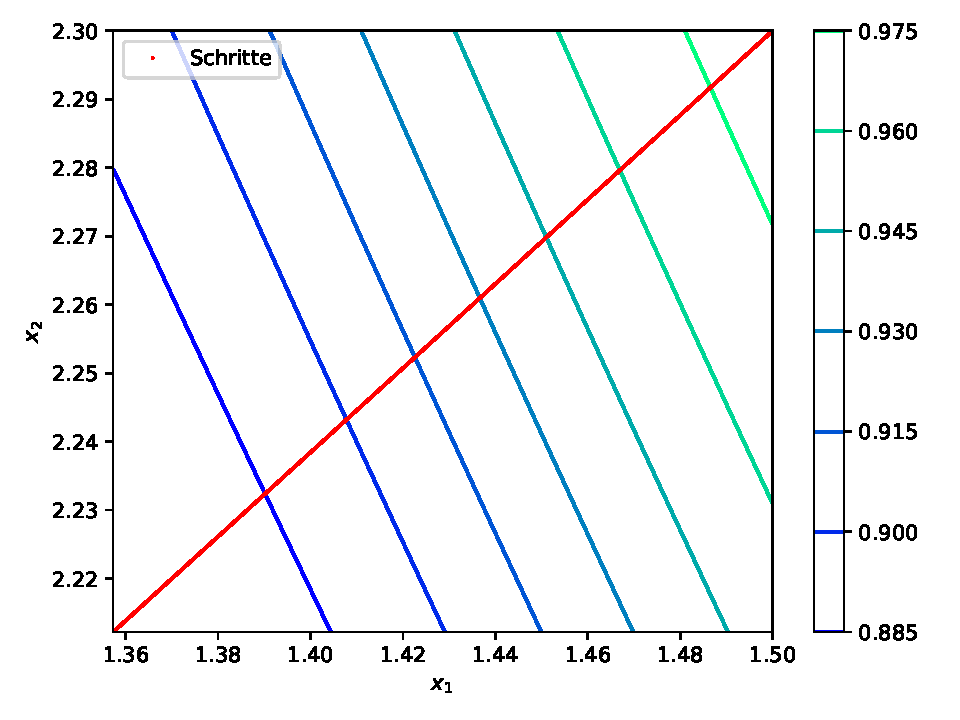
\includegraphics[width=0.45\textwidth]{A1/build/b1.pdf}
  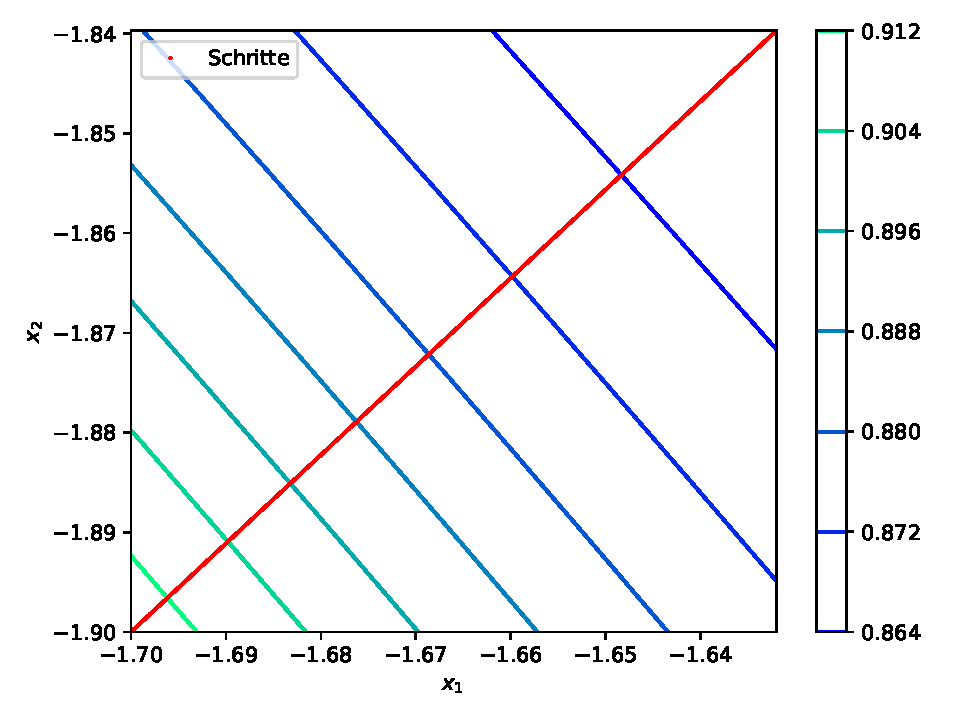
\includegraphics[width=0.45\textwidth]{A1/build/b2.pdf}
  \caption{Contour-Plot für den ersten (links) und zweiten Startwert (rechts).}
  \label{fig:contour_b}
\end{figure}
Es können möglicherweise auch noch andere lokale Minima existieren.
